%%%% ijcai09.tex

\documentclass{article}
% The file ijcai09.sty is the style file for IJCAI-09 (same as ijcai07.sty).
\usepackage{ijcai09}

% Use the postscript times font!
\usepackage{times}

% Set up graphics
\usepackage{graphicx}
\graphicspath{ {../graphs_and_data/} }

\usepackage{float}

% the following package is optional:
%\usepackage{latexsym} 

% Following comment is from ijcai97-submit.tex:
% The preparation of these files was supported by Schlumberger Palo Alto
% Research, AT\&T Bell Laboratories, and Morgan Kaufmann Publishers.
% Shirley Jowell, of Morgan Kaufmann Publishers, and Peter F.
% Patel-Schneider, of AT\&T Bell Laboratories collaborated on their
% preparation.

% These instructions can be modified and used in other conferences as long
% as credit to the authors and supporting agencies is retained, this notice
% is not changed, and further modification or reuse is not restricted.
% Neither Shirley Jowell nor Peter F. Patel-Schneider can be listed as
% contacts for providing assistance without their prior permission.

% To use for other conferences, change references to files and the
% conference appropriate and use other authors, contacts, publishers, and
% organizations.
% Also change the deadline and address for returning papers and the length and
% page charge instructions.
% Put where the files are available in the appropriate places.

\title{Inferring Gender from Audio Recordings}
\author{Jason Fairbourn, Mike Free, and Andrew Jensen \\
CS 478, Fall 2015\\
Department of Computer Science\\
Brigham Young University}

\begin{document}

\maketitle

\begin{abstract}
In this project, we investigate different methods of using machine learning to differentiate between recordings of male voices and female voices.  We begin by calculating the power cepstrum of each recording and using the cepstral coefficients as features.  After some initial results, we then investigate the effectiveness of the Mel Frequency Cepstral Coefficients (MFCC) as features.  We use this approach to generate data for several different learning models, ultimately discovering that KNN with a k-value of 1 produces the most accurate prediction accuracy.
\end{abstract}

\section{Introduction}

The field of speech recognition is broad and it could be said that it is still largely unsolved. Speech recognition has many different applications, from authentication to voice commands. Technology to recognize voice commands is beginning to enter mainstream devices with tools like Apple's Siri and Microsoft's Cortana.

In order to predict what a speaker says, signal processing techniques are used to analyze the audio recording of the command. These techniques generate features that are run through a learning model that attempts to label the instance. The features and labels depend on the application. For example, a voice command application would generate features related to vowel and consonant sounds, then predict common words that match the pattern in the features. A speaker recognition application - an application that recognizes and distinguishes the voices of various speakers - compares the generated features to labeled features of each speaker that exist in the training set.

In a speaker recognition problem, we can choose the type of application by the audio that we gather and the way we label it. We could build an application to recognize the sound of a single person’s voice by labeling recordings of that person as matches and multiple other people as non-matches. We could also build a more generic speaker recognition model by comparing one group of speakers with similar voices to another, for example, males and females. We chose to create a speaker recognition application to accomplish this task.

\section{Methods}

\subsection{Data Source}

In order to do gender recognition from speech, we needed to gather voice recordings of people saying some word or phrase. Initially, we decided that we would like to have at least a little consistency in our data, so we selected one type of high-quality microphone to train our model to: Olympus LS-3. In addition to having a consistent recording, we also wanted to have a consistent phrase.  We each went from door to door and from family gatherings to friend gatherings, collecting voice recordings of people saying the phrase "open sesame."

Though we did have some consistencies, we also wanted to have some variations so as to train our learning model well enough. We recorded each person three to five times, each time having them use different inflections. For example, we would ask the individual to say "open sesame" as a statement and then as a question. Another variation we introduced was background noise. We had a subset of recordings that were done at a family Thanksgiving event, which had some people talking in the background. We hoped that with these slight variations, we would be able to have enough data to allow our learning model to make the best guess possible. We decided to keep that subset of noisy data to further refine our choice of a learning model.

One potential problem that we were cautious about was the difference in ages of our speakers. A younger male boy could sound more like a female voice than a male one. So as a precaution, we also wrote down the ages of the individuals.

We ended up with 106 male recordings and 72 female recordings which is roughly a 60/40 split. Due to our current location, most of our recordings were of people within the college age range so the recording of ages turned out to be irrelevant with our data set.

\subsection{Initial Model}

In order to use machine learning to distinguish our audio files between male and female, we needed a way to extract relevant features from each recording.  To do this, we decided to use the power cepstrum, which provides a means to represent the rate of change in different frequency bands of an audio file.  It is calculated by taking the square of the absolute value of the Fourier transform of the audio signal, and then taking the inverse Fourier transform of the log of that result, and then finally taking the square of the absolute value of the resulting values to end up with the final power cepstrum.  In equation form, the power cepstrum is defined as follows:

$$
\left |{F}^{-1}\left \{log(\left |F\left \{f(t)\right \}\right |^2)\right \}  \right |^2 
$$

To apply this equation to each of our audio files, we created a Python script that parses through each file and uses the Numpy package to perform the required operations as defined above.  Our initial implementation would then store the first ten non-infinite coefficients as features for each audio file and either male or female as the classification (determined by the name of the directory that contained the file).  These features and classifications were then output to a file following standard .arff syntax.

Because of the model's success with predicting nominal classes from continuous features, we decided that we would use the Multi-Layer Perceptron as our initial testing model.  However, this model requires a large amount of input data in order to be effective, and since we were still in the process of manually collecting our data, we decided to use the Perceptron as an initial baseline estimate.  Once we had gathered enough data, we would then continue our experiments using the MLP model.

\section{Initial Results}

We began our initial experiments by testing the Perceptron model against the arff file generated by our initial Python script. Using 5-fold cross validation, we obtained the following result:

\begin{verbatim}
Calculating accuracy using
cross-validation...

Number of folds: 5
Fold=0, Accuracy=0.6666666666666666
Fold=1, Accuracy=0.5
Fold=2, Accuracy=0.25
Fold=3, Accuracy=1.0
Fold=4, Accuracy=1.0
Average time to train (in seconds): 0.0066
Mean accuracy=0.6833333333333333
\end{verbatim}

Repeating our test with different initial weights yielded similar results, and running our model with a 75/25 training/test split resulted in accuracies ranging from roughly 60\% to 80\%.  While these results appeared to perform better than a simple 50/50 guess, it was clear that further improvements needed to be made and we began investigating alternative feature extraction methods.

\section{Improvements}

\subsection{Data Refinement}

\subsubsection{Windowing}

An initial approach to improving the accuracy of our model was to break the power cepstrum into windowed segments and then taking the index of the highest cepstral coefficient for that segment.  We then attempted to calculate the original signal frequency that resulted in this coefficient, where the resulting frequency is the sampling rate divided by the coefficient index.  The top ten frequencies for each signal were then output as features in our resulting arff file.  Running this model through our perceptron using 10-fold cross validation resulted in the following:

\begin{verbatim}
Calculating accuracy using
cross-validation...
Number of folds: 10
Fold=0, Accuracy=1.0
Fold=1, Accuracy=0.5
Fold=2, Accuracy=0.5
Fold=3, Accuracy=0.0
Fold=4, Accuracy=0.0
Fold=5, Accuracy=1.0
Fold=6, Accuracy=1.0
Fold=7, Accuracy=0.5
Fold=8, Accuracy=0.0
Fold=9, Accuracy=0.5
Average time to train (in seconds): 0.0039
Mean accuracy=0.5
\end{verbatim}

As we can see, this approach did not significantly improve our model as expected.  In addition, 75/25 random splits also resulted in accuracies similar to what we had experienced previously (roughly 60\% to 80\%).  As such, we decided not to pursue this model any further.

\subsubsection{Mel-frequency Cepstral Coefficients (MFCC)}

We continued to research strategies for feature generation and learned about Mel-frequency Cepstral Coefficients. The mel scale (short for “melody”) is a logarithmic scale to map frequencies in such a way that pitches that are perceived as equally far apart are equally spaced on the scale. In other words, the mel scale converts pitches to a scale that more closely matches human hearing.

To generate Mel-frequency coefficients, we take the Fourier transform of the signal as the first step of generating the cepstrum, but we then map the frequencies from the result of the Fourier transform to the mel scale before we continue. This places the generated cepstral coefficients evenly apart in human hearing ranges. In a way, this makes our learning model "hear" the recordings the same way that a human hears them.

We used a python library that implements the Mel-frequency coefficient generation. We found that we could tweak how many coefficients it returned and decided that we would look further into the number of coefficients to use as features to find the best accuracy with different learning models if the MFCC provided any improvement - and it did.

We noticed a large improvement in accuracy by using MFCCs as features. Our simple Perceptron learner achieved 92\% training accuracy on the data set using 10-fold cross validation, where earlier methods of feature generation only achieved as high as 75\% accuracy.

\begin{figure}[H]
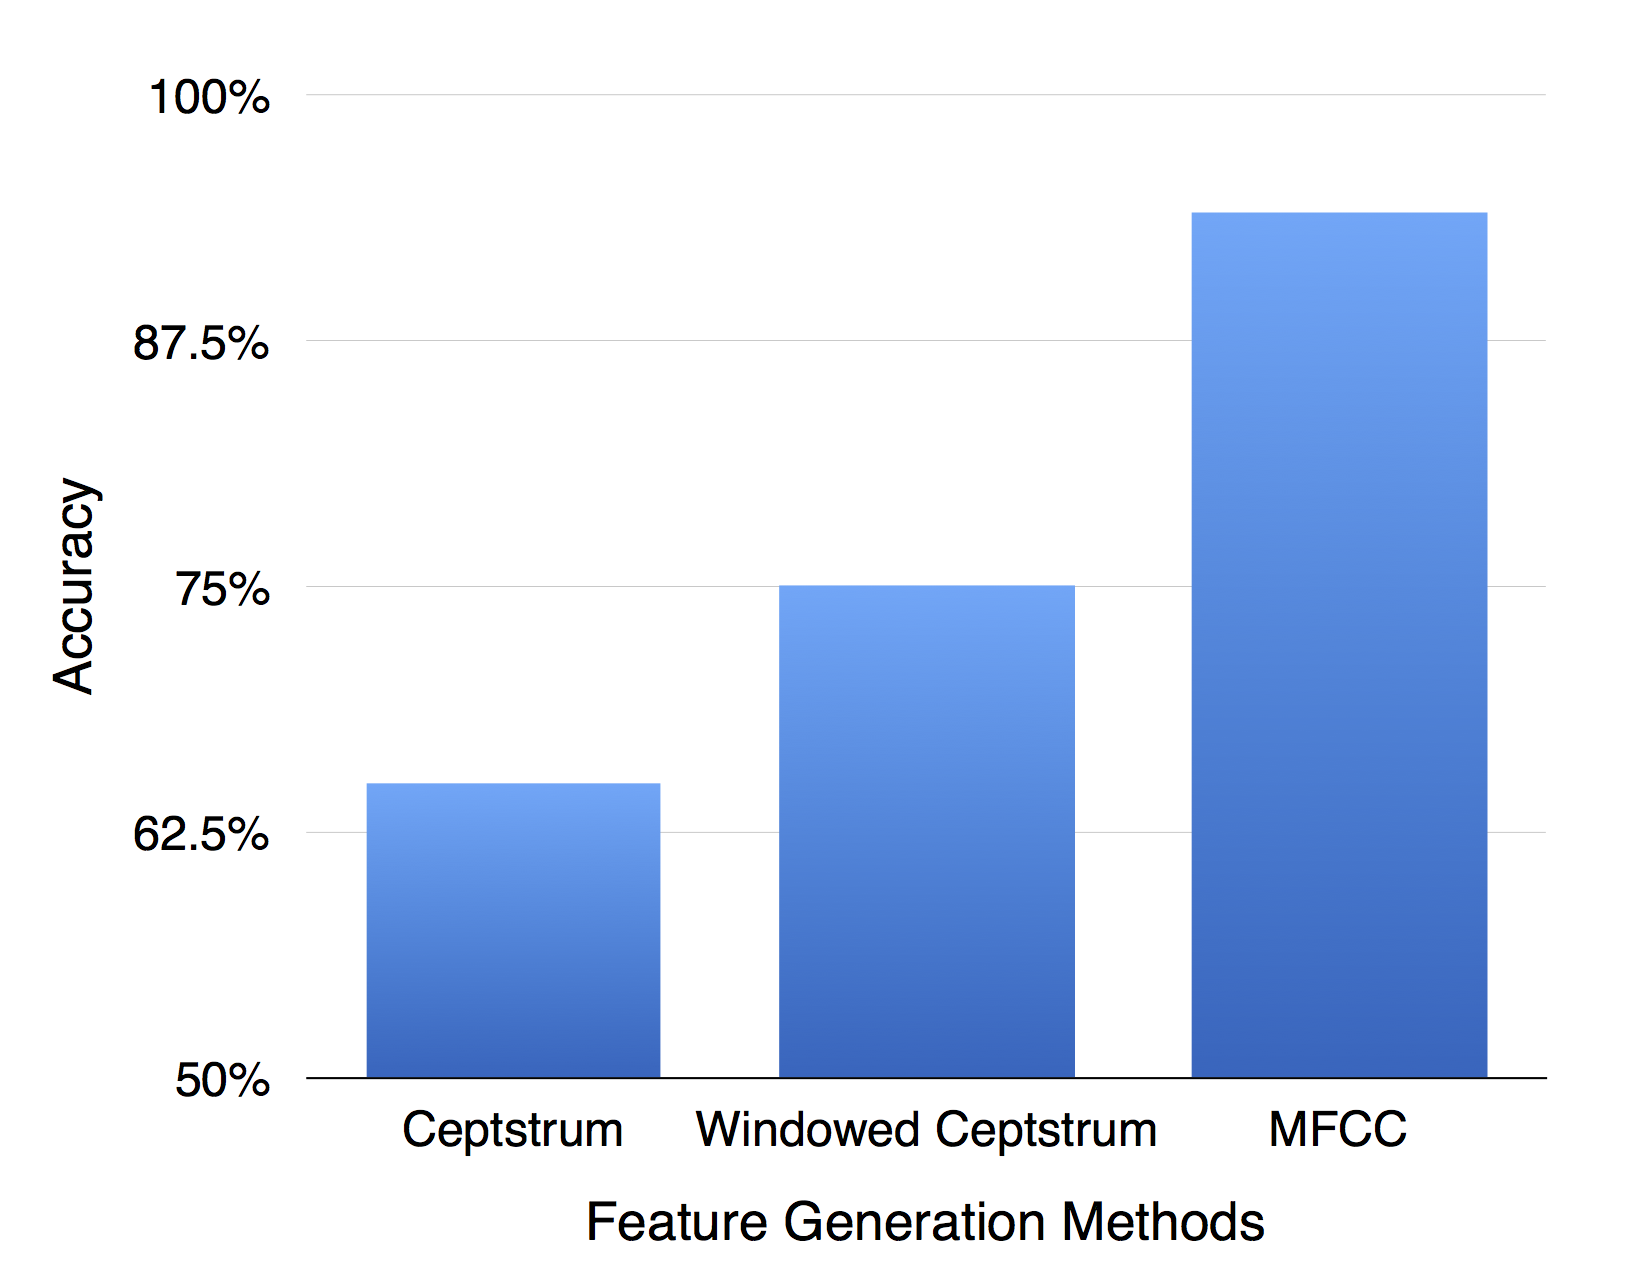
\includegraphics[width=\linewidth]{feature_generation_methods}
\end{figure}


\subsection{Learning Model Refinement}

We chose to use the Weka software to help us quickly select optimal learning models. We tried many different models including the Perceptron, VotedPerceptron, Multilayer Perceptron, Dagging, Hyperpipes, DecisionTable, and KNN. Below are the resulting accuracies using 10 fold cross validation for each of these models:

\begin{table}[H]
\centering
\caption{My caption}
\label{my-label}
\begin{tabular}{|l|l|}
\hline
Learning Model        & Accuracy \\ \hline
KNN                   & 98\%     \\ \hline
Multilayer Perceptron & 96\%     \\ \hline
Perceptron            & 93\%     \\ \hline
Dagging               & 90\%     \\ \hline
DecisionTable         & 83\%     \\ \hline
Hyperpipes            & 67\%     \\ \hline
VotedPerceptron       & 65\%     \\ \hline
\end{tabular}
\end{table}

Overall, we found that the Perceptron, MLP (learning rate 0.3, momentum 0.2), and KNN learning models performed the best and we decided to investigate and improve them further.

\subsubsection{Introduction of background noise}

As mentioned in 2.1, we gathered a subset of voice recordings done with some background noise. We were interested in seeing which of the three best-thus-far learning models would perform better when we introduced the background noise. We noted that without noise, the MLP and KNN learning models were nearly equal, but when we introduced the recordings with background noise, we found that the accuracy of MLP dropped significantly more than the KNN learning model from 98\% to 90\% while the KNN learning model had a 96\% accuracy.

\begin{figure}[H]
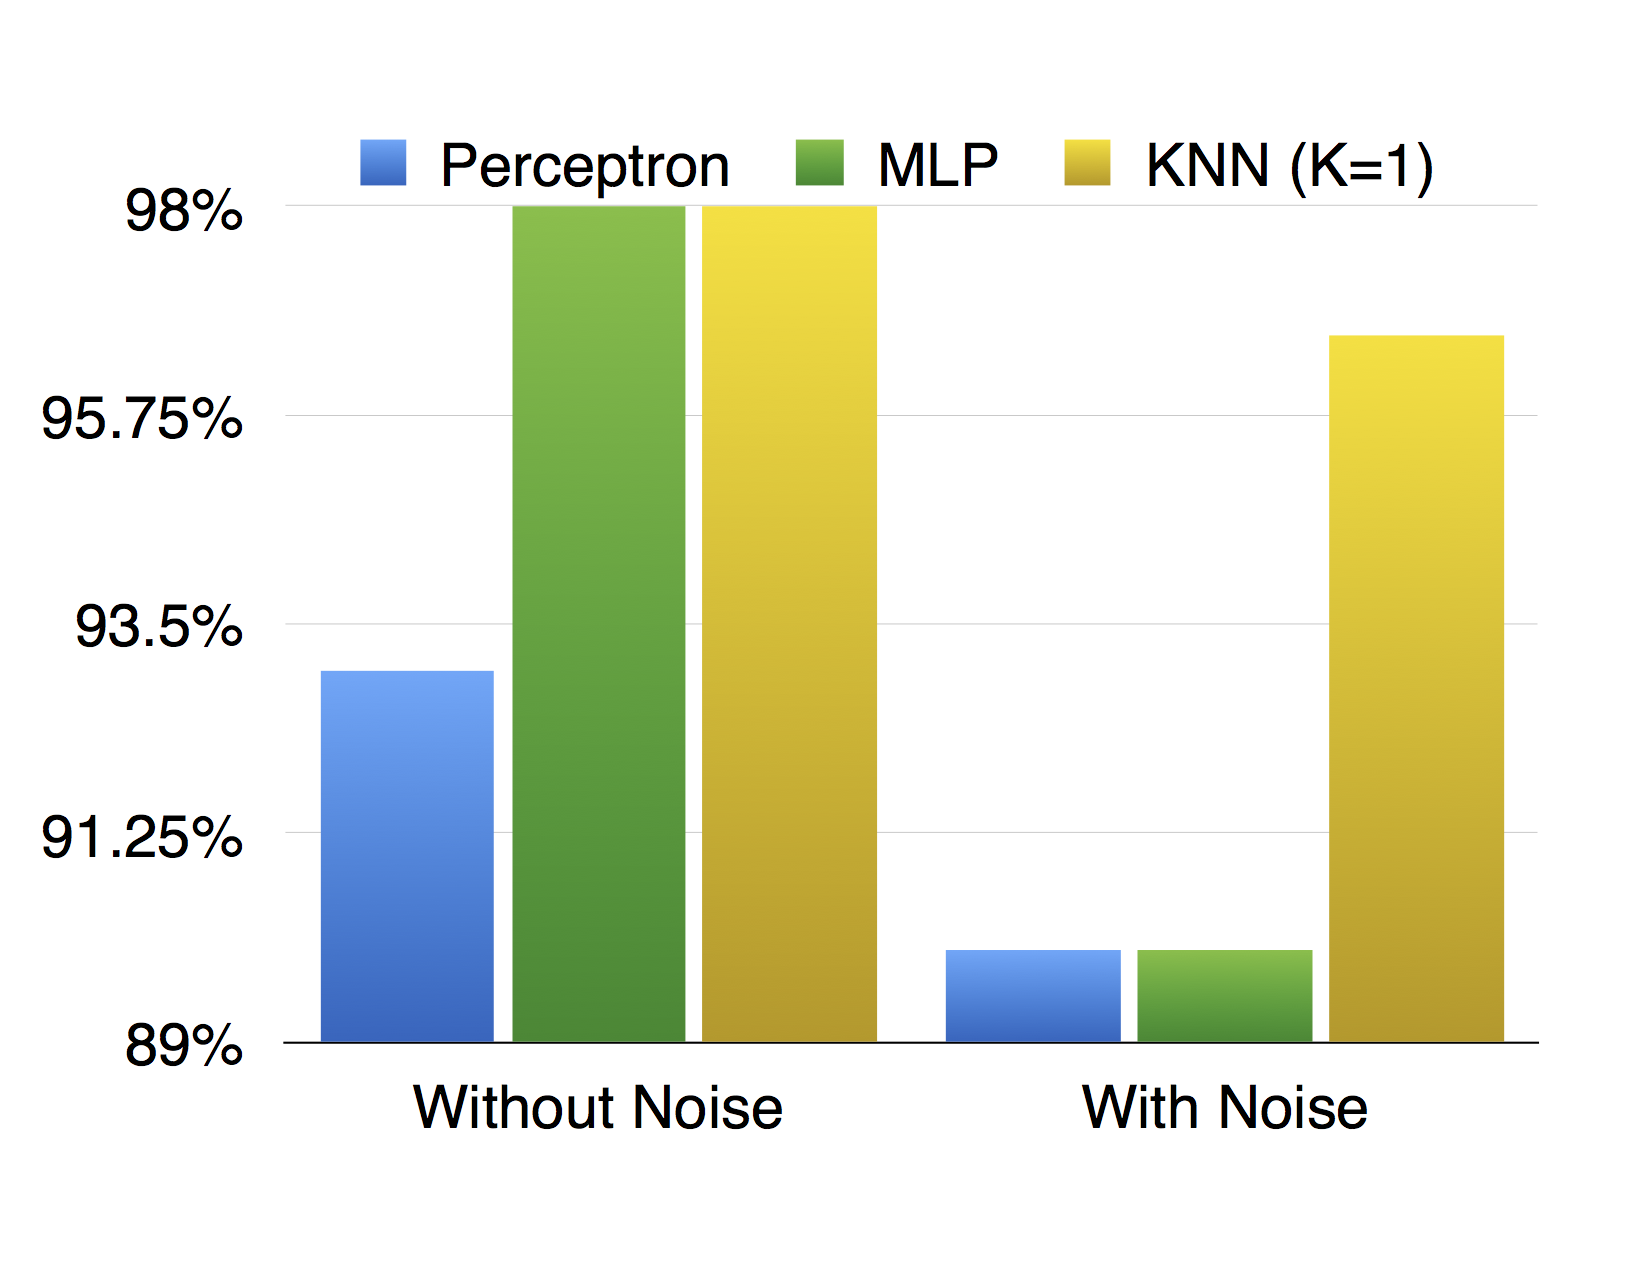
\includegraphics[width=\linewidth]{WithNoise_comparison}
\end{figure}

\subsubsection{Finding the optimal K for KNN}

We then decided to continue experimenting with KNN and try to determine the optimal value for K given our data set.  To do this, we carried out 10-fold cross validation tests with k-values of 1, 3, 5, and 7.  For each k-value, we also tested different amounts of cepstral coefficients used as features in the model.  These counts included 5, 10, 15, 20, and 25 coefficients.  This resulted in a total of 20 tests, the results of which are displayed in the following graph:

\begin{figure}[H]
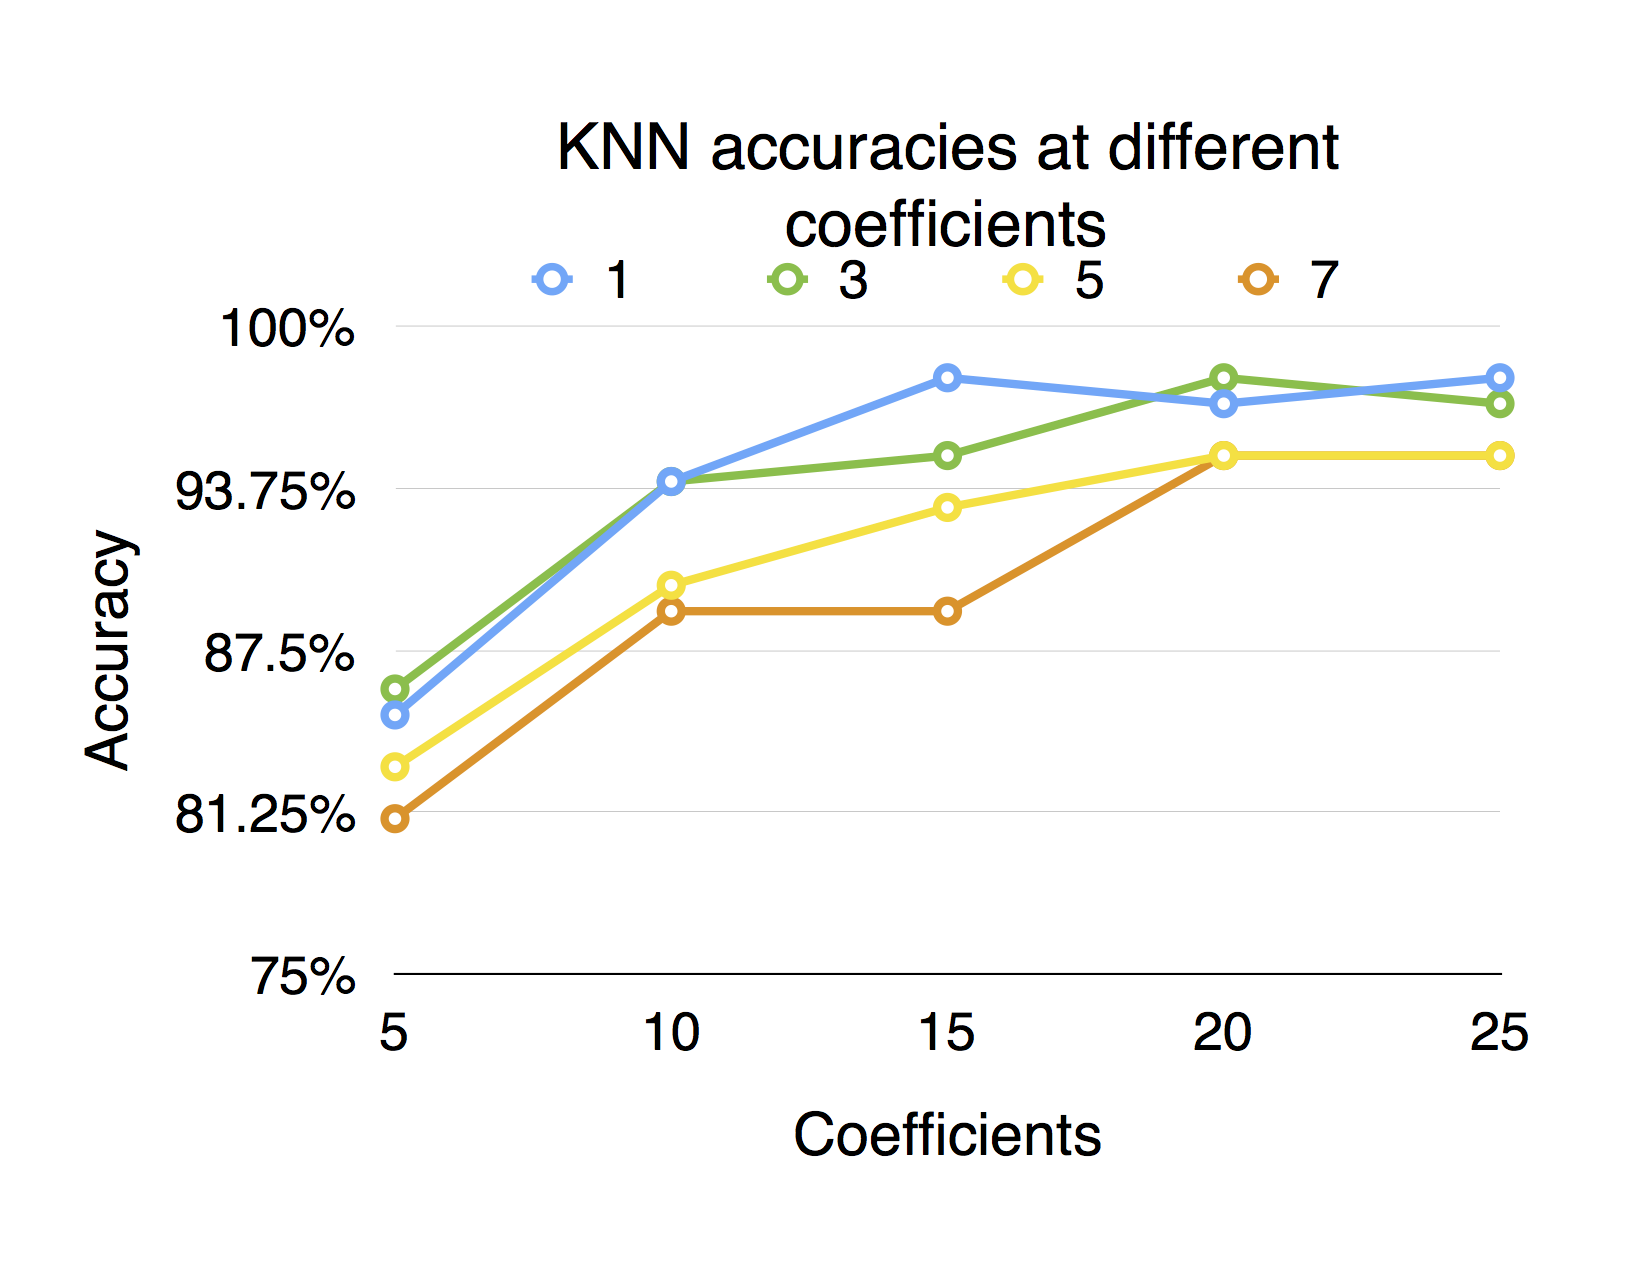
\includegraphics[width=\linewidth]{KNN_accuracies_with_different_coeff}
\end{figure}

It is interesting to note that an unusual pattern is emerging.  As we add more cepstral coefficients into our training data, the accuracy of the learning model increases, as opposed to decreasing as we initially expected.  In addition, it appears that k-values of 1 and 3 appear to be more accurate than other k-values.  While it is possible that this is explained by the fact that our training data contained 3-5 recordings of the same person, it is still interesting to observe that as more coefficients are used in the data, the more closely the model can represent gender based on the MFCC of the signal.

\section{Final Results and Conclusions}

Among all of our different learning models, all of them scored with a better accuracy than the baseline, which is 50\% - male or female. In the end, we found that the Perceptron, MLP, and KNN learning models scored the highest, each of them in the range of 88 to 98 percent.

\begin{figure}[H]
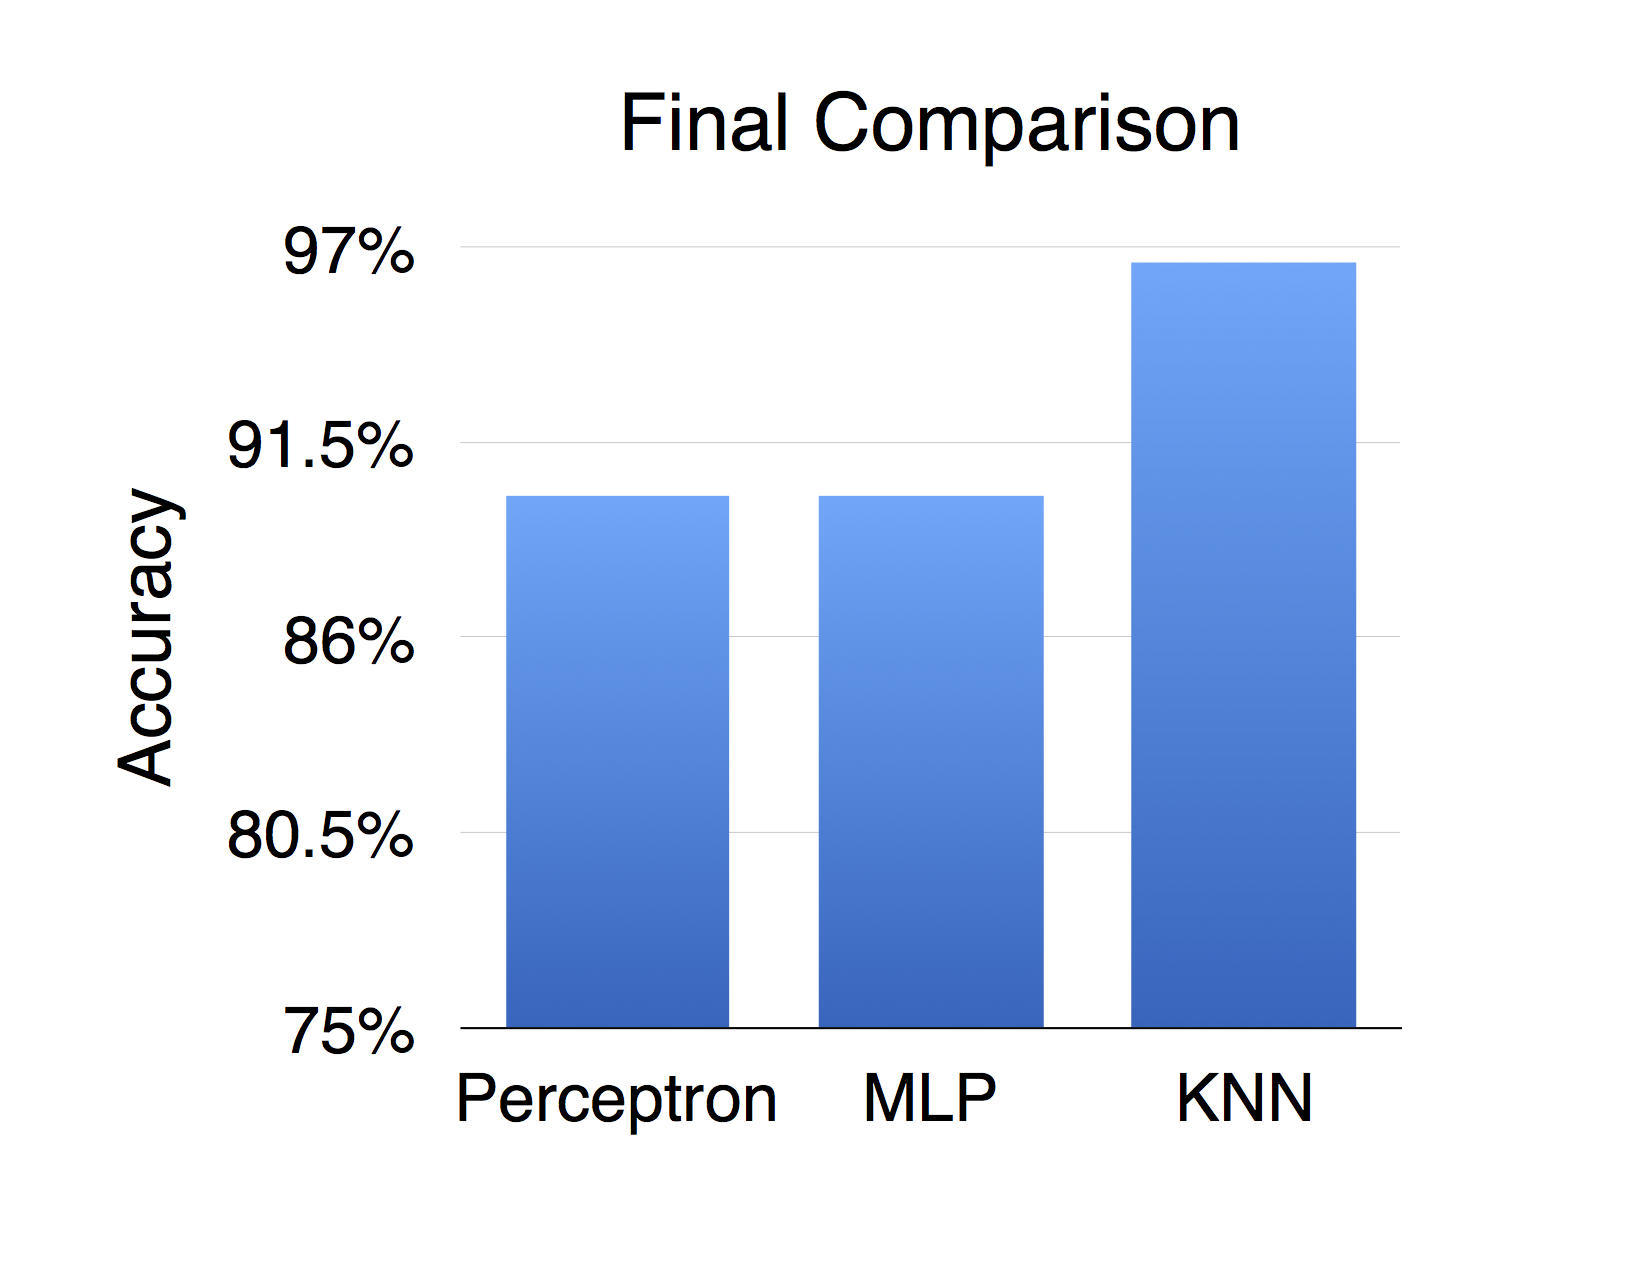
\includegraphics[width=\linewidth]{final_comparison}
\end{figure}

We believe that using the MFCC algorithm on our audio recordings was truly an essential part in increasing our prediction accuracy. Transforming the audio signals to a scale that matches human hearing caused our perceptron learning model to jump from 75\% to 93\%. 

It seemed like we had a clear winner with KNN where K = 1 when we introduced recordings with background noise; however, it was pointed out to us afterwards that perhaps the three to five recordings of each person could have been the cause of the KNN model working better with our 10 fold cross validation method. Essentially, we were training our model with a few of the 3-5 recordings per person and testing with the rest. This would certainly have an effect on our test set accuracies and perhaps our choice of K for KNN. With more time, we would like to improve our accuracy results with a more "pure" test set. If upon improving our test set we discover that KNN doesn't prove to be as good, we would also try to gather more voice recordings to help improve the Multilayer Perceptron model.

\section{Future Work}

When we took on this project, we knew that there would be more ways to extend this idea of predicting gender from speech. What if we could detect the ages of an individual based on their speech? Knowing both the gender and the age of an individual could play a major part in relevant searches and ads.

We would also like to explore the idea of doing speaker recognition in order to unlock mobile phones or other locks. We believe this is very possible, but we would also like to see if we could catch any attempt to forge a person's voice, i.e. using a recording of a person to unlock his phone.

In this project, we tried to control certain aspects of the data gathering by using a specific voice recording device. Lower quality microphones would introduce more noise to the data, so making our model more robust to these recordings would be another problem to solve. We'd like to gather recordings from microphones on mobile phones and computers and see how that affects our accuracy. One thing that we could do is synthesize random noise in all of our recordings and try to find ways to eliminate that noise.

The current trends in technology going on in the world right now are putting more and more focus on signal processing. With these ideas of future work to be done, we hope to assist in merging signal processing with machine learning to improve our world.

\appendix


%% The file named.bst is a bibliography style file for BibTeX 0.99c
\nocite{*}
\bibliographystyle{named}
\bibliography{ijcai09}

\end{document}

